% *********************************************************************
% © 2016–2025 Jeremy Sylvestre
%
% Permission is granted to copy, distribute and/or modify this document
% under the terms of the GNU Free Documentation License, Version 1.3 or
% any later version published by the Free Software Foundation; with no
% Invariant Sections, no Front-Cover Texts, and no Back-Cover Texts. A
% copy of the license is included in the appendix entitled “GNU Free
% Documentation License” that appears in the output document of this
% PreTeXt source code. All trademarks™ are the registered® marks of
% their respective owners.
%
% *********************************************************************
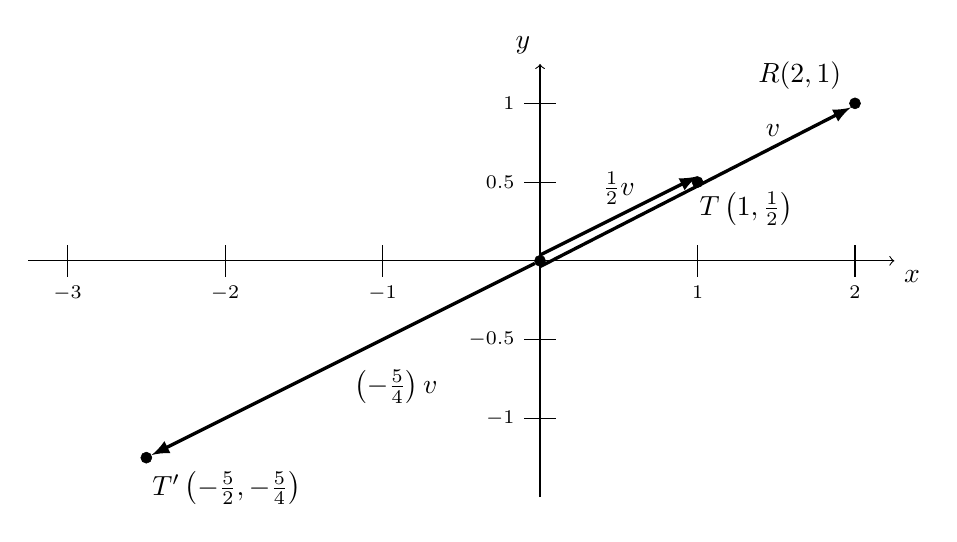
\begin{tikzpicture}[
	point/.style={circle,draw,very thin,fill,inner sep=0pt,minimum size=4pt},
	vector/.style={-latex},
	scale=2
]

	% (1/2)x
%	\begin{scope}[yscale=1.5]
		\draw[->] (-3.25,0) to (2.25,0) node[below right] {$x$};
		\draw[->] (0,-1.5) to (0,1.25) node[above left] {$y$};
		\foreach \x in {-3,-2,-1,1,2} {
			\draw (\x,0.1) to (\x,-0.1) node[below] {$\scriptstyle \x$};
		}
		\foreach \y in {-1,-0.5,0.5,1} {
			\draw (0.1,\y) to (-0.1,\y) node[left] {$\scriptstyle \y$};
		}
		\node[point] at (0,0) (o) {};
		\node[point] at (2,1) (r) [label=above left:{$R(2,1)$}] {};
		\node[point] at (1,0.5) (t) [label={[xshift=-0.15cm,yshift=0.05cm]below right:{$T\left(1, \frac{1}{2}\right)$}}] {};
		\node[point] at (-2.5,-1.25) (t2) [label={[xshift=-0.1cm]below right:{$T'\left( -\frac{5}{2}, -\frac{5}{4} \right)$}}] {};
		\draw[vector,very thick] (o.south) to node[above,near end] {$\uvec{v}$} (r.south west);
		\draw[vector,very thick] (o.north) to node[above] {$\frac{1}{2} \uvec{v}$} (t.north);
		\draw[vector,very thick] (o) to node[below right] {$\left(-\frac{5}{4}\right) \uvec{v}$} (t2);
%	\end{scope}

\end{tikzpicture}
